

Mithilfe von Scopes oder Plots werden nun die gesuchten Signale abgegriffen und als Funktionen der Zeit dargestellt. \\
Die Abbildungen \ref{fig:Moment}, \ref{fig:Omega} und \ref{fig:StreckeundUnwuchtkraft} sind Plots aus Matlab, die wie folgt definiert wurden:

\begin{figure}[hbt]
	\centering
	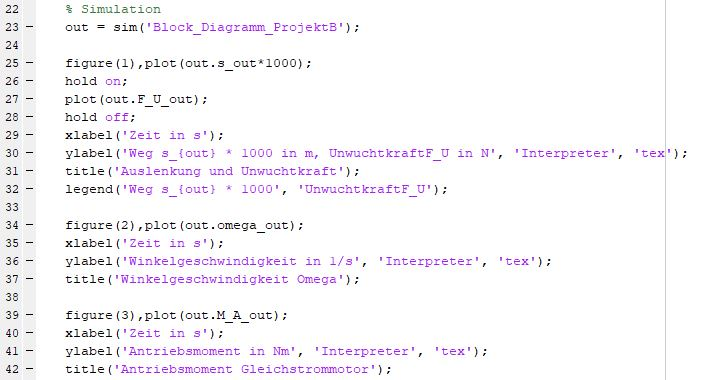
\includegraphics[width=1\linewidth]{Images/Simulationscode}
	\caption{}
	\label{fig:Simcode}
\end{figure}

In den folgenden Abbildungen \ref{fig:Moment}, \ref{fig:Omega} und \ref{fig:StreckeundUnwuchtkraft} sind das Motormoment $M$, die Winkelgeschwindigkeit $\Omega$, die Strecke $s$ und die Unwuchtkraft $F_U$ über die Zeit von $100 \milli\second$ dargestellt.

\begin{figure}[hbt]
	\centering
	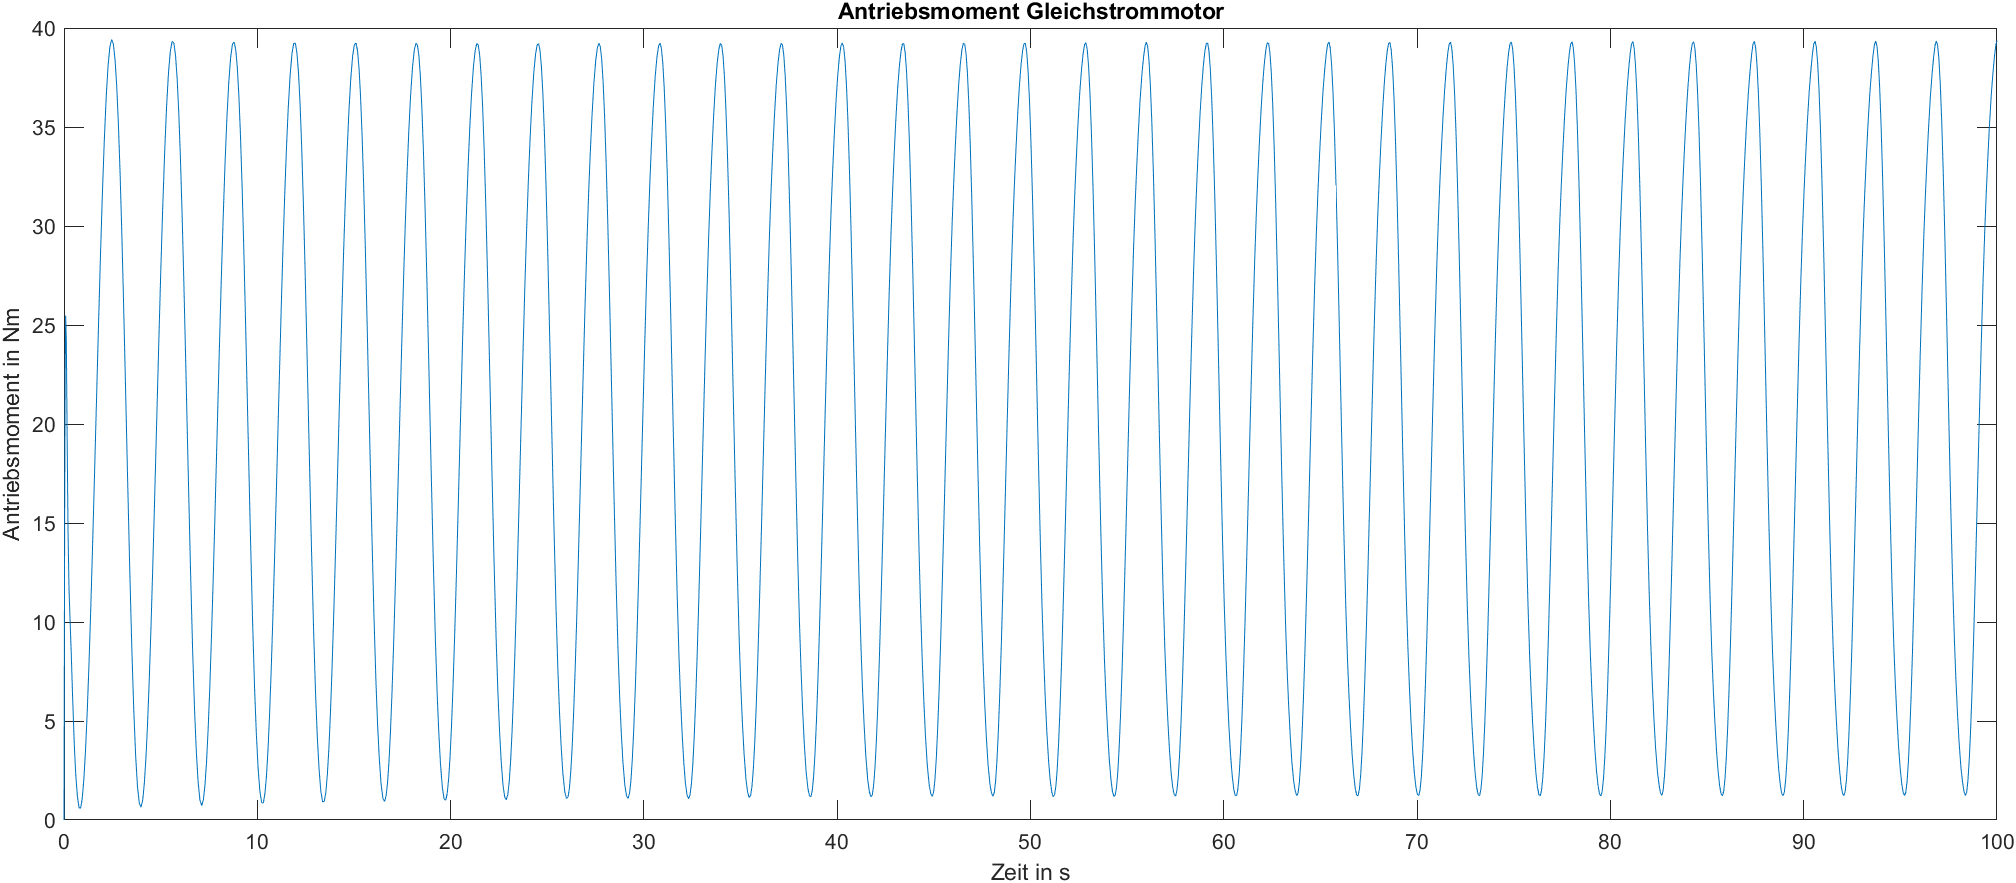
\includegraphics[width=1\linewidth]{Images/Moment}
	\caption{Simulationsergebnis: Antriebsmoment des Gleichstrommotors}
	\label{fig:Moment}
\end{figure}

\begin{figure}[hbt]
	\centering
	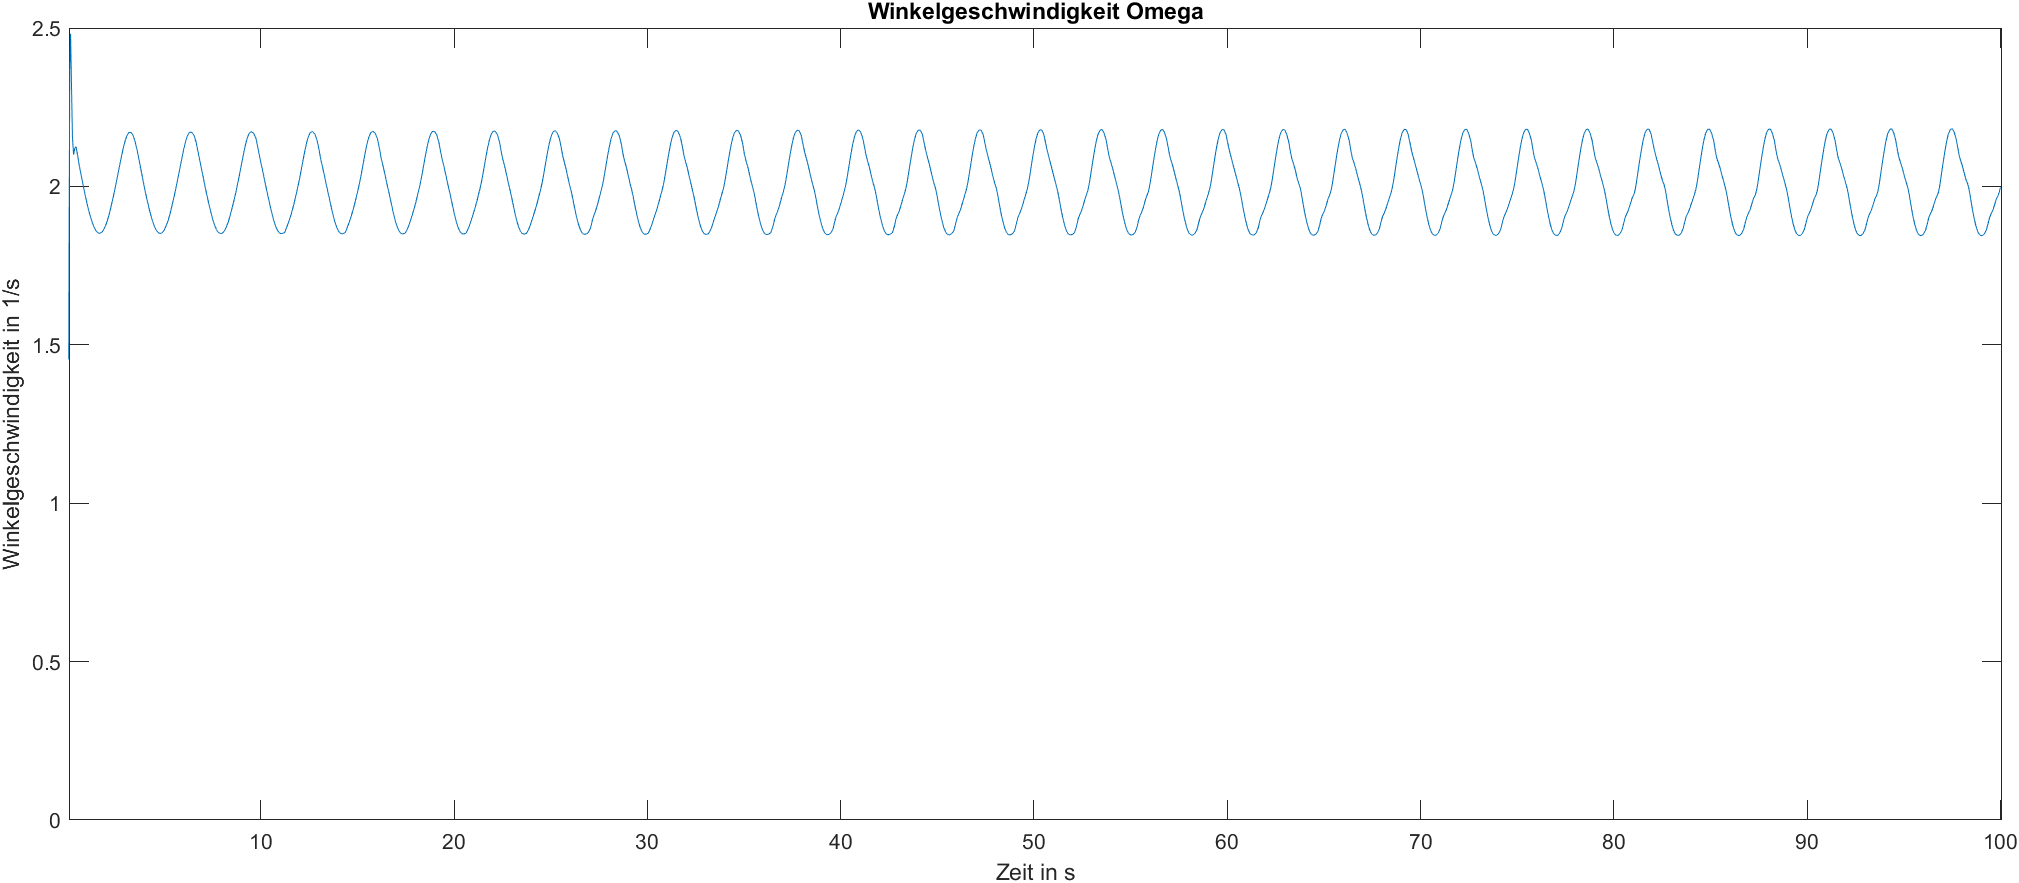
\includegraphics[width=1\linewidth]{Images/Omega}
	\caption{Simulationsergebnis: Winkelgeschwindigkeit des mechatronischen Systems}
	\label{fig:Omega}
\end{figure}

Auffällig ist in Abbildung \ref{fig:StreckeundUnwuchtkraft}, dass die Auslenkung die doppelte Frequenz der Unwuchtkraft hat.

\begin{figure}[hbt]
	\centering
	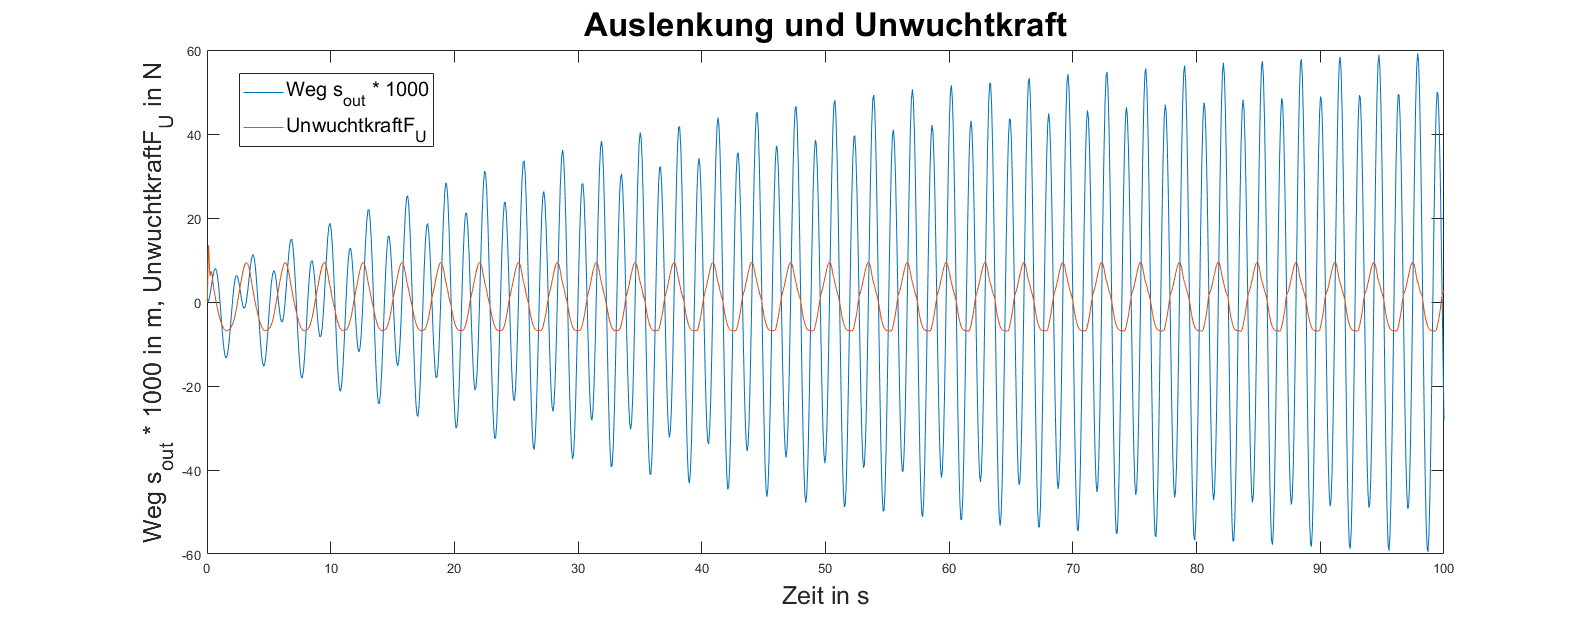
\includegraphics[width=1\linewidth]{Images/StreckeundUnwuchtkraft}
	\caption{Simulationsergebnis: Auslenkung$\cdot$1000 und Unwuchtkraft des mechatronischen Systems}
	\label{fig:StreckeundUnwuchtkraft}
\end{figure}



